\documentclass{beamer}
\usepackage{pgfpages}
%%\setbeameroption{show notes on second screen=left} %enable for notes
\usepackage{graphicx}
\usepackage{xcolor}
\usepackage{listings}
\usepackage{hyperref}
\lstset{language=python,frame=single}
\usepackage{verbatim}
\usepackage{apacite}
\usepackage{subcaption}
\usepackage{amsmath}
\usepackage{relsize}
\usepackage{appendixnumberbeamer}
\usepackage{xparse}
\usepackage{multimedia}
\usepackage{tikz}
\usetikzlibrary{matrix,backgrounds}
\pgfdeclarelayer{myback}
\pgfsetlayers{myback,background,main}

\tikzset{mycolor/.style = {line width=1bp,color=#1}}%
\tikzset{myfillcolor/.style = {draw,fill=#1}}%

\NewDocumentCommand{\highlight}{O{blue!40} m m}{%
\draw[mycolor=#1,rounded corners] (#2.north west)rectangle (#3.south east);
}

\NewDocumentCommand{\fhighlight}{O{blue!40} m m}{%
\draw[myfillcolor=#1,rounded corners] (#2.north west)rectangle (#3.south east);
}

\usetheme[numbering=fraction]{metropolis}
%%\AtBeginSection[]
%%{
%%  \begin{frame}
%%    \frametitle{Table of Contents}
%%    \tableofcontents[currentsection]
%%  \end{frame}
%%}

%%\let\olditem\item
%%\renewcommand{\item}{\vspace{0.5\baselineskip}\olditem}
\begin{document}

\title{Learning Parallels}
\subtitle{Analogies emerge from learning dynamics in neural networks}
\author{Andrew Lampinen}
\date{FriSem, 3/24/2017}
\frame{\titlepage}


\section{Introduction}
\begin{frame}{Last time...}
\begin{center}
\includegraphics[width = 0.66\textwidth]{../../../fyp/figures/fyp_1_polygon_text.png}
\end{center}
\begin{center}
\includegraphics[width = 0.66\textwidth]{../../../fyp/figures/fyp_1_modular_text.png}
\end{center}
\note{Both transfer effects of presentation on later concepts, and effects of learning two analogous instantiations of the same concept. Today, we're going to take a step back and explore *MODELING* some of these more general phenomena}
\end{frame}

%%TODO Outline

%%TODO: Plot?
\begin{frame}{Analogy, Transfer, and Cognition}
A variety of perspectives:
\begin{itemize}
    \item<1-> ``What makes humans smart is (1) our exceptional ability to learn by analogy'' \cite{Gentner2003} 
    \item<2-> ``Significant transfer is probably rare and accounts for very little human behavior. ... We generally do what we have learned to do and no more.'' \cite{Detterman1993}
    \item<3-> ``We found evidence for analogical transfer from a concrete, highly perceptual system to a very dissimilar domain and task ... participants' transfer was independent of their explicit reports [of awareness of the analogy between the tasks].'' \cite{Day2011}
    \item<4-> ``Our proposal is to view transfer from the perspective of preparation for future learning (PFL).'' \cite{Bransford1999} 
\end{itemize}
\note{Fortunately, there's a great deal of agreement in the field. What is the driving force? One possibility (which Bransford \& Schwartz among others acknowledged) is that there are different kinds of transfer. Failures to transfer most often occur in settings like Gick \& Holyoak's experiments with the Duncker radiation problem, where participants see one example and then have to do a symbolic mapping to another example. By contrast, successful analogical transfer often occurs in situations like Day \& Goldstone's, where participants actually interact with the system and learn about it over a period of time, or more generally in education as highlighted by Bransford \& Schwartz as the ability to learn faster in the future.}
\end{frame}

\begin{frame}{Analogy, Transfer, and Cognition}
Why the disagreement?
\begin{itemize}
    \item<2-> Different kinds of analogy/transfer:
\end{itemize}
\uncover<3->{
\begin{center}
\begin{table}
\begin{tabular}{|c|c|}
\hline 
Fast & Slow \\
\hline
\parbox{0.45\textwidth}{
\begin{itemize}
\item<4-> one (or a few) examples explicitly shown
\item<5-> transfer requires explicit awareness of analogy 
\end{itemize} 
}
&
\parbox{0.45\textwidth}{
\begin{itemize}
\item<4-> learning through many interactions
\item<5-> transfer need not be explicit 
\end{itemize}
}\\ \hline 
\end{tabular}
\end{table} 
\end{center}
}
\uncover<6->{In this talk we'll focus on the ``slow'' type, which we think could explain much of the analogical reasoning that supports everyday cognition (e.g. preparation for learning).}
\end{frame}

%%\begin{frame}{Analogy, Transfer, and Cognition}
%%Why is fast transfer rare?
%%\begin{itemize}
%%    \item<2-> Finding analogies symbolically is hard! (How many possible analogies are there?)  
%%\end{itemize}
%%\uncover<3->{Why is slow transfer more common?}
%%\begin{itemize}
%%    \item<4-> \textbf{Is finding analogies implicitly ``easy''?}
%%\end{itemize}
%%\end{frame}


\begin{frame}{Analogy, Transfer, and Neural Networks}
Neural networks:
\begin{itemize}[<+->]
    \item Can show cross-task transfer
    \begin{itemize}
	\item Transfer in artificial grammar learning \cite{Dienes1999}
	\item Multi-task learning, zero-shot generalization \cite{Luong2016,Johnson2016}  
    \end{itemize}
    \item Can show representation of analogies
    \begin{itemize}
	\item Verbal analogies \cite{Kollias2013}
	\item Extract analogous structure from non-overlapping tasks \cite{Hinton1986}.
    \end{itemize}
\end{itemize}
\only<1>{\vspace{-14pt}}
\note{Cross-task transfer without building it in!}
\end{frame}

\begin{frame}{Hinton family-tree task}
\begin{columns}
\column{0.5\textwidth} Q: ``Who is Arthur's mother?'' \\ A: ``Penelope'' %\\[11pt] Q: ``Who is Emilio's mother?'' \\ A: ``Maria'' 
\column{0.5\textwidth}
    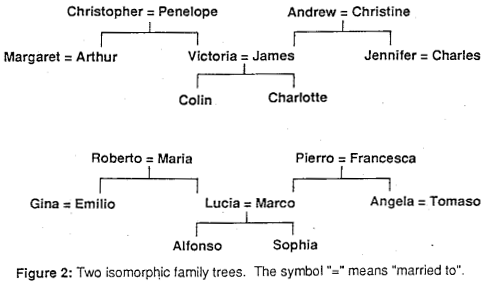
\includegraphics[width = \textwidth]{../writing/cogsci_2017/figures/hinton_family_tree_figure.png}
\end{columns}
\uncover<2->{Do neural networks naturally extract analogies?}
\end{frame}

\begin{frame}{Analogy, Transfer, and Neural Networks}
Our claims:
\begin{itemize}
    \item<1-> Neural networks learning by gradient descent naturally extract analogies. 
    \item<2-> This happens in more general circumstances than shown in previous work, in particular it does not rely on shared weights.
    \item<3-> This could act as a form of amortized inference about analogies which could drive transfer (and could potentially serve as a search heuristic explicit analogical reasoning).
\end{itemize}
\end{frame}

\section{Modeling: A toy task}
\begin{frame}{A toy task}
Learning which letters can follow other letters:\vspace{-2em}
\begin{center}
\[
%%\begin{array}{c|cccccc} 
%%& P & D & S & \pi & \delta & \sigma \\
%%\hline
%%R & 1 & 1 & 0 & 0 & 0 & 0 \\
%%L & 1 & 0 & 1 & 0 & 0 & 0 \\
%%\rho & 0 & 0 & 0 & 1 & 1 & 0\\
%%\lambda & 0 & 0 & 0 & 1 & 0 & 1\\
%%\end{array} 
\begin{array}{c|cccc} 
& R & L & \rho & \lambda \\
\hline
P & 1 & 1 & 0 & 0 \\ 
D & 1 & 0 & 0 & 0 \\
S & 0 & 1 & 0 & 0 \\
\pi    & 0 & 0 & 1 & 1 \\ 
\delta & 0 & 0 & 1 & 0 \\
\sigma & 0 & 0 & 0 & 1 \\
\end{array} 
\]
\end{center}
\uncover<2->{How, when, and why will a neural network exploit the analogy between the Latin and Greek letters?}
\end{frame}

\section{(A Little) Theory}
\begin{frame}
Neural networks are difficult to interpret.
\end{frame}


\begin{frame}{SVD Analyses?}
Easier to interpret: linear neural networks!
\only<1>{\vspace{-16pt}}
\begin{columns}
\column{0.5\textwidth}
\begin{itemize}
    \item<8-> Learning is driven entirely by features of the SVD (Singular Value Decomposition) of the Input/Output (I/O) mapping \cite{Saxe2013}.
    \item<9-> Analyzing the SVD can tell us about the structure the network is actually learning. 
\end{itemize}
\column{0.5\textwidth}
    \only<1>{\vspace{16pt}}
    \begin{overlayarea}{\textwidth}{0.5\textheight}
    \only<1>{\includegraphics[width=\textwidth]{figures/linear_network_diagram_blank.png}}
    \only<2>{\includegraphics[width=\textwidth]{figures/R_forward_1.png}}
    \only<3>{\includegraphics[width=\textwidth]{figures/R_forward_2.png}}
    \only<4>{\includegraphics[width=\textwidth]{figures/R_forward_3.png}}
    \only<5>{\includegraphics[width=\textwidth]{figures/rho_forward_1.png}}
    \only<6>{\includegraphics[width=\textwidth]{figures/rho_forward_2.png}}
    \only<7->{\includegraphics[width=\textwidth]{figures/rho_forward_3.png}}
    \end{overlayarea}
\end{columns}
\note{SVD is way of factorizing a matrix into ``modes'', you can think of these kind of like components in PCA, they're ordered in terms of ``how much variance they explain.'' }
\end{frame}


%%TODO: border around modes? Do not zero center
\begin{frame}{SVD Analyses?}
SVD breaks down the structure of the task into ``modes'' that together explain the data (like components in PCA).
\begin{figure}
\centering
\begin{subfigure}{0.22\textwidth}
\includegraphics[width=\textwidth]{./figures/nonlinear_IO.png}
%\caption{$\Sigma_{IO}$}
\end{subfigure}
{\!\!\huge{$=$}\!\!}
\begin{subfigure}{0.22\textwidth}
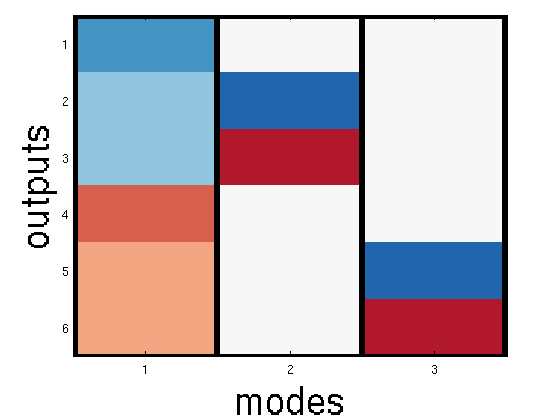
\includegraphics[width=\textwidth]{./figures/U_nl.png}
%\caption{$U$}
\end{subfigure}
{\!\!\LARGE{$\times$}\!\!}
\begin{subfigure}{0.22\textwidth}
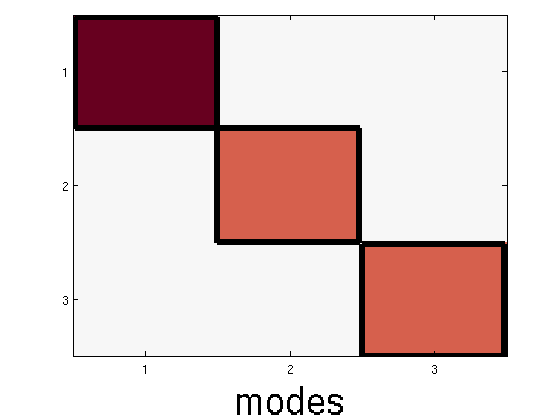
\includegraphics[width=\textwidth]{./figures/S_nl.png}
%\caption{$S$}
\end{subfigure}
{\!\!\LARGE{$\times$}\!\!}
\begin{subfigure}{0.22\textwidth}
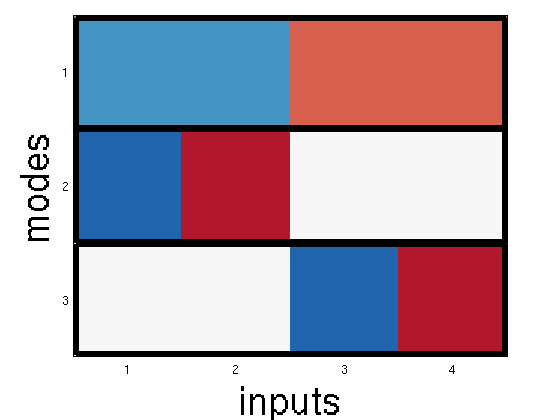
\includegraphics[width=\textwidth]{./figures/V_nl.png}
%\caption{$V^T$}
\end{subfigure}
\end{figure}
\uncover<2->{This allows us to learn more about what the network is actually doing to solve the task.}
\note{Really talk through SVD, first component gving strong separation between domains, and the letter that's ``always on'' in each language, second two components give within domain structure. Analyzing the SVD is more principled than just looking at weights or hidden unit activations, because it is more invariant to rotations of representation space, etc.}
\end{frame}

\begin{frame}{SVD Analyses?}
Can we use SVD analyses of linear networks to study analogy learning?
\begin{itemize}
    \item<1-> \textbf{NO,} in the SVD of a block-diagonal matrix, the modes occur within the blocks, thus \textbf{a linear network cannot represent analogies at convergence.}
    \uncover<2->{
    \begin{figure}
    \centering
    \begin{subfigure}{0.2\textwidth}
    \includegraphics[width=\textwidth]{./figures/nonlinear_IO.png}
    %\caption{$\Sigma_{IO}$}
    \end{subfigure}
    {\!\!\huge{$=$}\!\!}
    \begin{subfigure}{0.2\textwidth}
    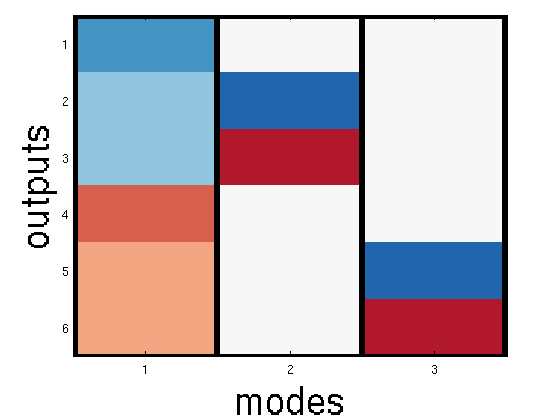
\includegraphics[width=\textwidth]{./figures/U_nl.png}
    %\caption{$U$}
    \end{subfigure}
    {\!\!\LARGE{$\times$}\!\!}
    \begin{subfigure}{0.2\textwidth}
    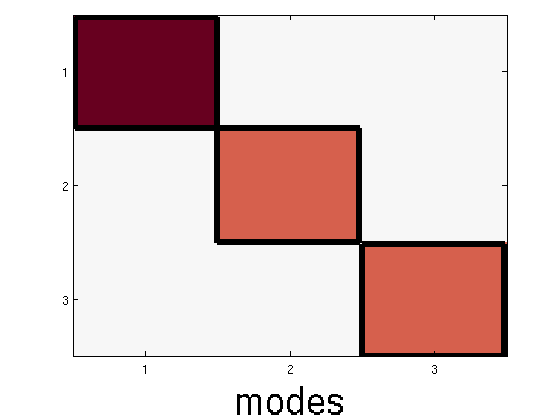
\includegraphics[width=\textwidth]{./figures/S_nl.png}
    %\caption{$S$}
    \end{subfigure}
    {\!\!\LARGE{$\times$}\!\!}
    \begin{subfigure}{0.2\textwidth}
    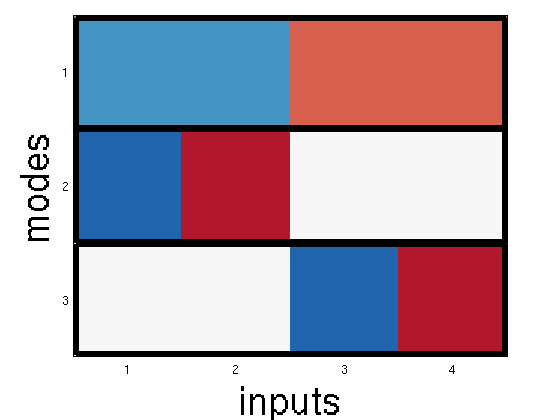
\includegraphics[width=\textwidth]{./figures/V_nl.png}
    %\caption{$V^T$}
    \end{subfigure}
    \end{figure}
    }
    \item<3-> This also means that a linear network \textbf{cannot achieve as parsimonious a solution as a nonlinear network}, because it must solve each copy of a problem separately rather than exploiting analogies between them.
\end{itemize}
\note{In plain english, what this means is the input output mappings for the two tasks are not really connected in any way, the most naive way to solve the task where you solve each problem independently.}
\end{frame}

\begin{frame}{Linearized analysis}
So we need non-linear networks. \uncover<2->{Is there a way we can still use SVD analyses?} 
\begin{itemize}
\item<3-> \textbf{Yes}, with a single non-linearity, just analyze linear portion.
\end{itemize}
\only<1>{ \includegraphics[width=0.83\textwidth]{figures/network_with_nothing.png}}
\only<2>{ \includegraphics[width=0.83\textwidth]{figures/network_with_QM.png}}

\note{Yes, just put a non-linearity at the end and apply to the linear portion}
\end{frame}

\section{That's enough theory -- back to the task results}
%%\begin{frame}{Toy task}
%%What solutions does the network discover? \\[11pt]
%% \includegraphics[width=0.83\textwidth]{figures/network_with_IO_and_QM.png}
%%\note{note that no weights are shared between the two tasks!}
%%\end{frame}

\begin{frame}{Toy task results}
Most commonly, the network learns an (offset) analogy structure:\\[11pt] 
\begin{overlayarea}{\textwidth}{0.5\textheight}
\only<1>{\includegraphics[width=\textwidth]{figures/network_with_IOs.png}}
\only<2->{
\[
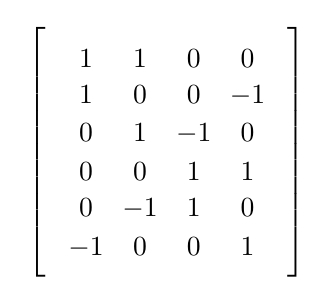
\begin{tikzpicture}[ampersand replacement=\&]
\matrix(m)[matrix of math nodes,left delimiter={[},right delimiter={]}] 
{ 
 1 \& 1 \& 0 \& 0 \\ 
 1 \& 0 \& 0 \& -1 \\
 0 \& 1 \& -1 \& 0 \\
 0 \& 0 \& 1 \& 1 \\ 
 0 \& -1 \& 1 \& 0 \\
 -1 \& 0 \& 0 \& 1 \\
};

\begin{pgfonlayer}{myback}
\fhighlight[red!30]{m-1-1}{m-3-2}
\fhighlight[red!30]{m-4-3}{m-6-4}
\fhighlight[blue!30]{m-1-3}{m-3-4}
\fhighlight[blue!30]{m-4-1}{m-6-2}
\end{pgfonlayer}
\end{tikzpicture}
\]
}
\end{overlayarea}
\uncover<3->{(This is certainly not the only solution that can occur, but this happens about 75\% of the time. The remaining 25\% no analogy is discovered.)}
\end{frame}

\begin{frame}{Comparing SVDs}
\begin{itemize}
    \item<1-> Earlier: 
    \uncover<1->{
    \begin{figure}
    \centering
%%    \begin{subfigure}{0.2\textwidth}
%%    \includegraphics[width=\textwidth]{../writing/cogsci_2017/figures/nonlinear_IO.png}
%%%%    \caption{$\Sigma_{IO}$}
%%    \end{subfigure}
%%    \raisebox{0.5em}{\!\!\huge{$=$}\!\!}
    \begin{subfigure}{0.25\textwidth}
    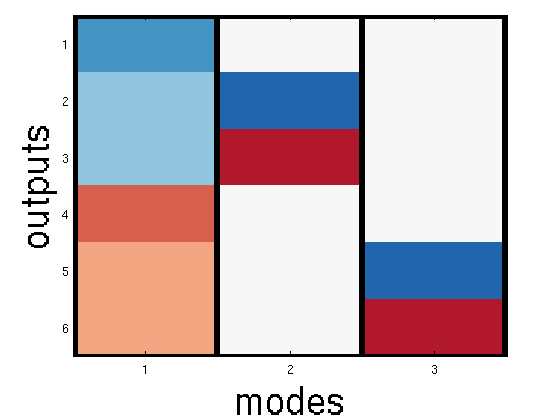
\includegraphics[width=\textwidth]{./figures/U_nl.png}
%%    \caption{$U$}
    \end{subfigure}
    \raisebox{0.5em}{\!\!\LARGE{$\times$}\!\!}
    \begin{subfigure}{0.25\textwidth}
    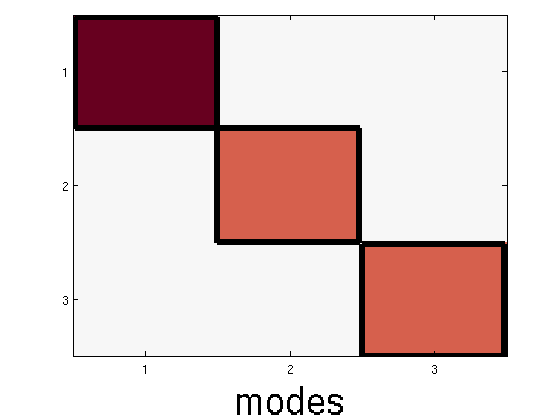
\includegraphics[width=\textwidth]{./figures/S_nl.png}
%%    \caption{$S$}
    \end{subfigure}
    \raisebox{0.5em}{\!\!\LARGE{$\times$}\!\!}
    \begin{subfigure}{0.25\textwidth}
    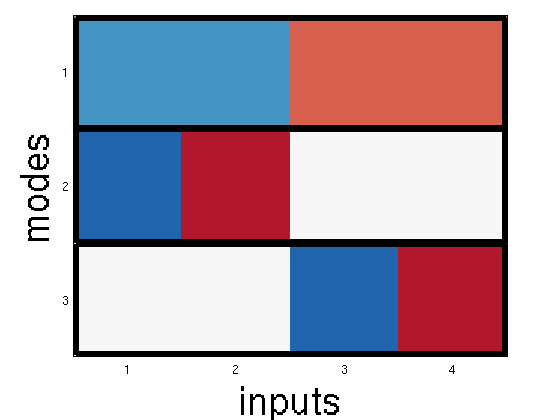
\includegraphics[width=\textwidth]{./figures/V_nl.png}
%%    \caption{$V^T$}
    \end{subfigure}
    \end{figure}
    }
    \item<2-> Now:
    \uncover<2->{
    \begin{figure}
    \centering
%%    \begin{subfigure}{0.25\textwidth}
%%    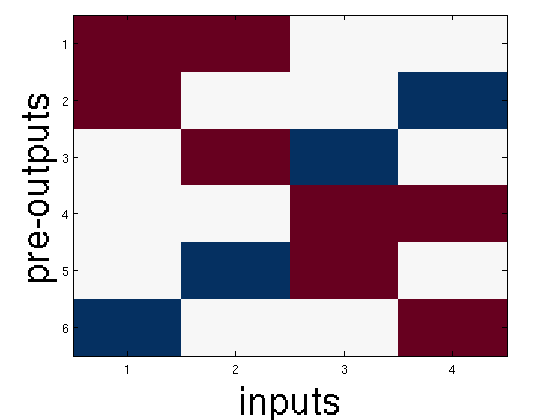
\includegraphics[width=\textwidth]{../writing/cogsci_2017/figures/linearized_IO.png}
%% %%   \caption{$\Sigma_{IO}$}
%%    \end{subfigure}
%%    \raisebox{0.5em}{\!\!\huge{$=$}\!\!}
    \begin{subfigure}{0.25\textwidth}
    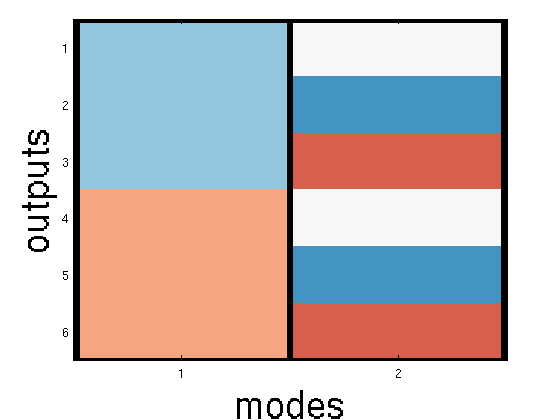
\includegraphics[width=\textwidth]{./figures/U_lz.png}
%%    \caption{$U$}
    \end{subfigure}
    \raisebox{0.5em}{\!\!\LARGE{$\times$}\!\!}
    \begin{subfigure}{0.25\textwidth}
    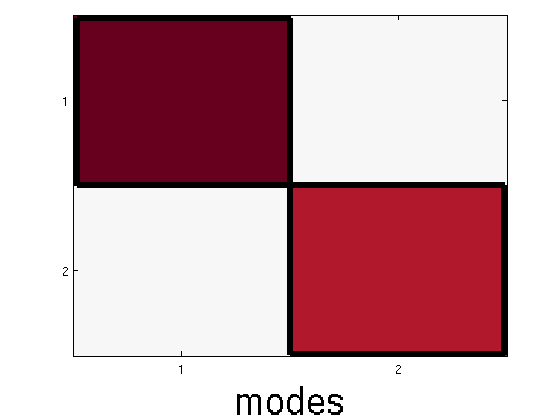
\includegraphics[width=\textwidth]{./figures/S_lz.png}
%%    \caption{$S$}
    \end{subfigure}
    \raisebox{0.5em}{\!\!\LARGE{$\times$}\!\!}
    \begin{subfigure}{0.25\textwidth}
    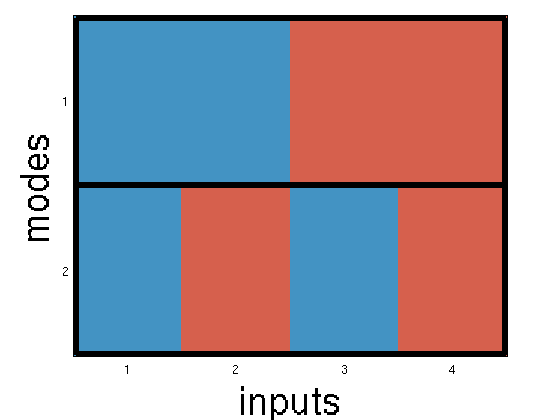
\includegraphics[width=\textwidth]{./figures/V_lz.png}
%%    \caption{$V^T$}
    \end{subfigure}
    \end{figure}
    }
    \item<3-> Network has captured the analogy!
    \item<4-> Results in more parsimonious solution (lower-rank, fewer hidden units neeeded).
\end{itemize}
\note{Can interpret the top SVD in several ways, as the task that a linear network solves, or as the task that a non-linear network begins solving when it is still in the linear regime. Note more parsimonious solutions available with linearized mapping -- i.e. lower rank.}
\end{frame}

%%\begin{frame}{Learning dynamics}
%%But when and how does this occur? The linearized SVD cannot tell us about learning dynamics, but the progression is fairly consistent: \\[11pt]
%%\begin{columns}
%%    \column{0.45\textwidth}
%%    \uncover<2->{Initial:{\relsize{-1}
%%    \[ 
%%    \left[ \begin{matrix} 
%%    0 & 0 & 0 & 0 & 0 & 0 \\
%%    \vdots & \vdots &\vdots &\vdots &\vdots &\vdots \\
%%     0 & 0 & 0 & 0 & 0 & 0\\
%%    \end{matrix}  \right] 
%%    \] 
%%    }}
%%    \uncover<4->{Base rates by domain:{\relsize{-1}
%%    \[
%%    \left[ \begin{matrix} 
%%    1 & 0.5 & 0.5 & 0 & 0 & 0 \\
%%    1 & 0.5 & 0.5 & 0 & 0 & 0 \\
%%    0 & 0 & 0 & 1 & 0.5 & 0.5  \\
%%    0 & 0 & 0 & 1 & 0.5 & 0.5  \\
%%    \end{matrix}  \right] 
%%    \]
%%    }
%%    }
%%    \column{0.45\textwidth}
%%    \uncover<3->{Base rates:{\relsize{-1}
%%    \[ 
%%    \left[ \begin{matrix} 
%%    0.5 & 0.25 & 0.25 & 0.5 & 0.25 & 0.25 \\
%%    \vdots & \vdots &\vdots &\vdots &\vdots &\vdots \\
%%     0.5 & 0.25 & 0.25 & 0.5 & 0.25 & 0.25\\
%%    \end{matrix}  \right] 
%%    \] 
%%    }}
%%    \uncover<5->{Solution with offsets:{\relsize{-1}
%%    \[
%%    \left[ \begin{matrix} 
%%    1 & 1 & 0 & 0 & 0 & -1 \\
%%    1 & 0 & 1 & 0 & -1 & 0 \\
%%     0 & 0 & -1 & 1 & 1 & 0\\
%%     0 & -1 & 0 & 1 & 0 & 1\\
%%    \end{matrix}  \right] 
%%    \]
%%    }}
%%\end{columns}
%%\uncover<6->{For all but the last step, linear network learning dynamics are very similar! Do linear networks also show any signs of analogical learning?}
%%\note{base rates by domain = first component of SVD}
%%\end{frame}
\section{Learning dynamics}
\begin{frame}{Learning dynamics}
In fact, linear networks begin to extract the analogy as well, but must discard it to achieve their optimal solution.
\begin{center}
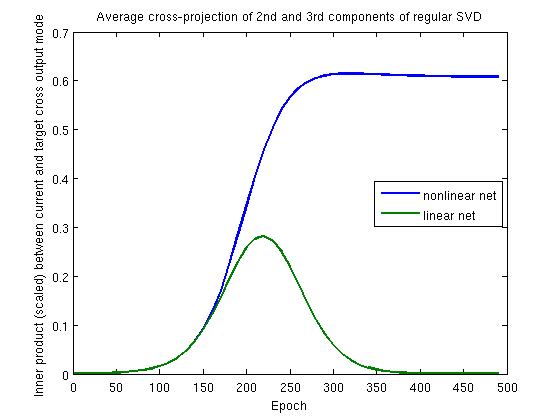
\includegraphics[width=0.7\textwidth]{../writing/cogsci_2017/figures/SVD_cross_projection_learning.png}
\end{center}
\end{frame}

\begin{frame}{Learning dynamics}
Why? When gradually learning analogous tasks simultaneously, extracting the analogy reduces error. \\[11pt]
\begin{columns}
    \column{0.45\textwidth}
    \uncover<1->{Base rates by domain: \phantom{a little shared structure}{\relsize{-1}
    \[
    \left[ \begin{matrix} 
     1 & 1 & 0 & 0 \\ 
     0.5 & 0.5 & 0 & 0 \\
     0.5 & 0.5 & 0 & 0 \\
     0 & 0 & 1 & 1 \\ 
     0 & 0 & 0.5 & 0.5 \\
     0 & 0 & 0.5 & 0.5 \\
    \end{matrix}  \right] 
    \]
    }
    \begin{center}\textbf{MSE = 0.5}\end{center}}
    \column{0.45\textwidth}
    \uncover<1->{Base rates + a little shared structure{ \relsize{-1}
    \[
    \left[ \begin{matrix} 
     1 & 1 & 0 & 0 \\ 
     0.6 & 0.4 & 0.1 & -0.1 \\
     0.4 & 0.6 & -0.1 & 0.1 \\
     0 & 0 & 1 & 1 \\ 
      0.1 & -0.1 & 0.6 & 0.4 \\
      -0.1 & 0.1 & 0.4 & 0.6 \\
    \end{matrix}  \right] 
    \] 
    }
    \begin{center}\textbf{MSE = 0.34}\end{center}}
\end{columns} 

\note{So network will exploit the analogy to reduce error, even though no weights are shared, and even if it must discard it in the linear case.}
\end{frame}

\section{Interim summary}
\begin{frame}{Interim summary}
 In this simple task:
\begin{itemize}
    \item<2-> Representation of the analogy emerges naturally from the learning dynamics because it reduces error.
    \item<3-> This occurs in about 75\% of random initializations.
    \item<4-> This does not depend on shared weights, gradually learning two analogous tasks simultaneously suffices.
    \item<5-> Thus it seems that neural networks could provide amortized inference about analogies. 
\end{itemize}
\uncover<6->{But is this only because the task was simple?}
\end{frame}

\section{A more interesting example: Hinton's family tree task}
\begin{frame}{Hinton family tree task}
\begin{columns}
    \column{0.5\textwidth}
    \begin{center}
	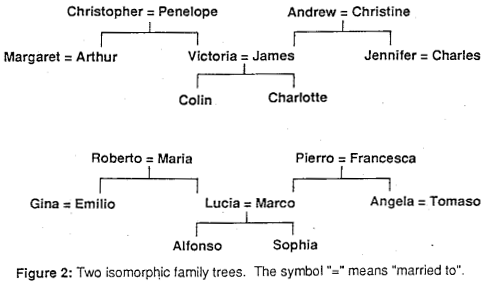
\includegraphics[width = \textwidth]{../writing/cogsci_2017/figures/hinton_family_tree_figure.png}
    \end{center}
    \column{0.5\textwidth}
    \uncover<2-> {
    \begin{center}
	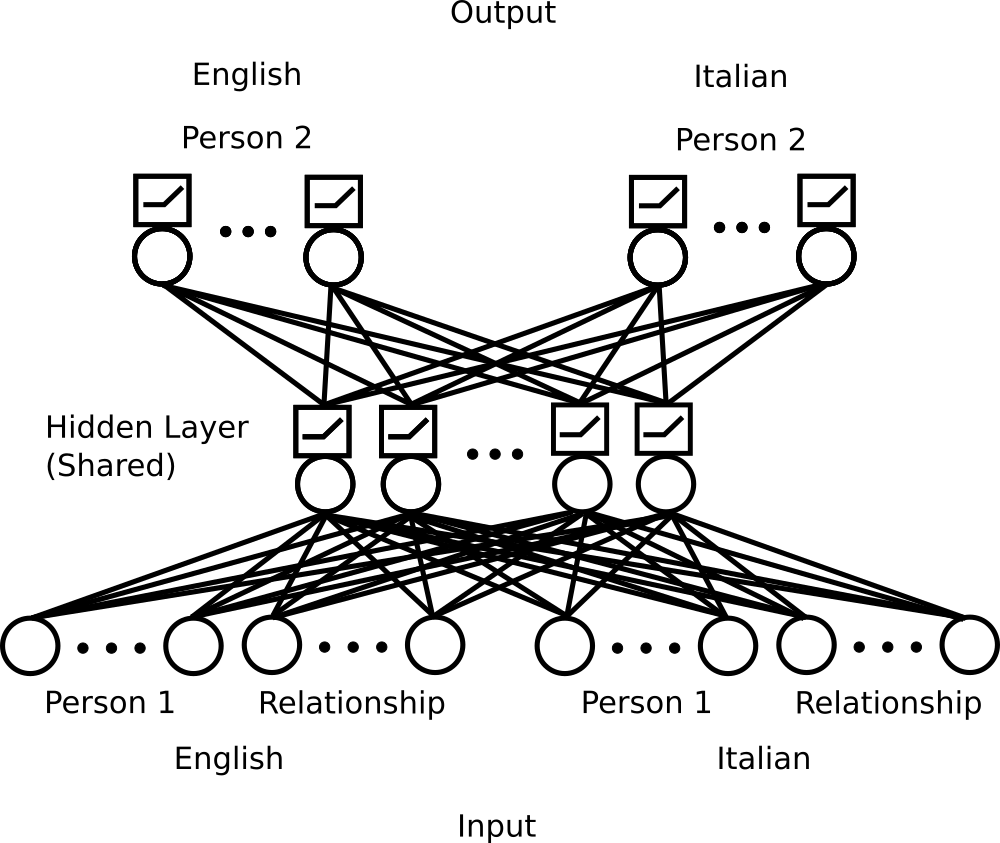
\includegraphics[width = \textwidth]{../writing/cogsci_2017/figures/family_tree_network_diagram.png}
    \end{center}
    }
\end{columns}
\uncover<2-> {
\begin{itemize}
\item Our network is simplified from Hinton's -- has no shared weights and tasks are completely separated.
\end{itemize}
}
\end{frame}

\begin{frame}{Hinton family tree task: Problems}
A few problems:
\begin{itemize}
    \item<1-> Task is not linearly separable, so we have multiple non-linearities, so how to perform analysis?
    \begin{itemize}
	\item<2-> The simple approach we took is just to perform the linearized analysis at each layer. 
    \end{itemize}
    \uncover<2-> {
    \begin{center}
	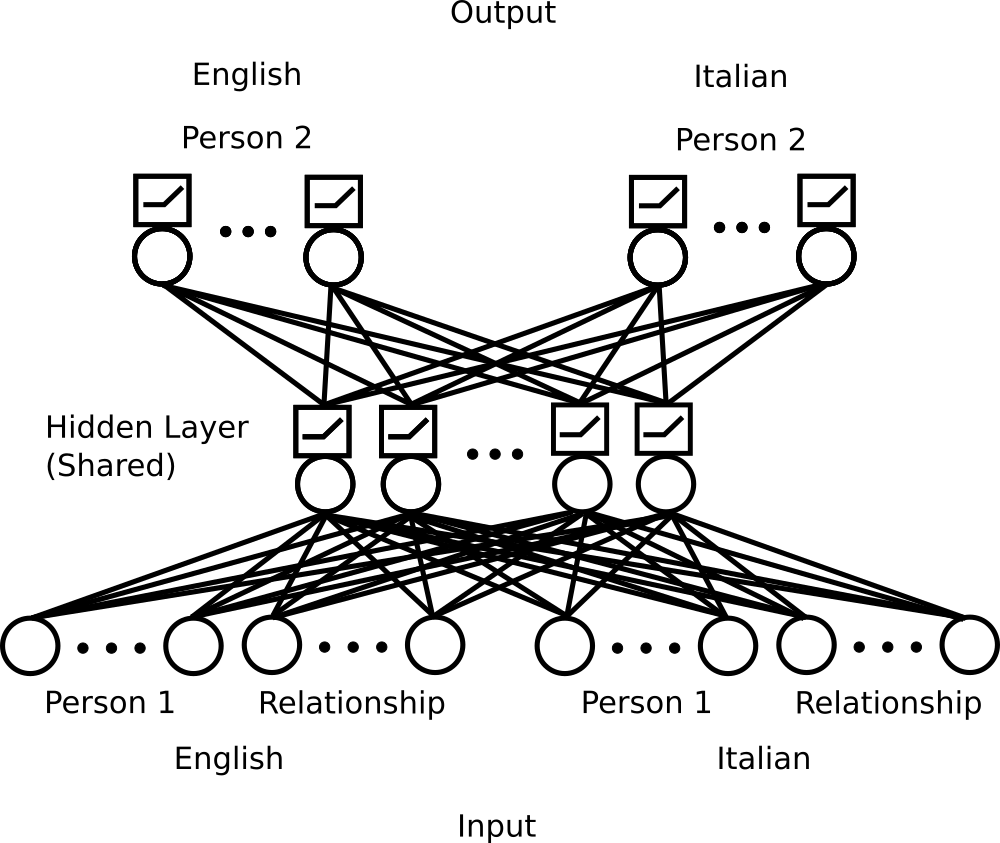
\includegraphics[width = 0.5\textwidth]{../writing/cogsci_2017/figures/family_tree_network_diagram.png}

    \end{center}
    }
\end{itemize}
\note{Hinton shared relationship inputs, and had shared hidden layers, but we want to strip down to see if the analogies will emerge from the learning dynamics like in the above task.}
\end{frame}

\begin{frame}{Hinton family tree task: Problems}
A few problems:
\begin{itemize}
    \item<1-> Multiple analogies exist between family trees (for example flip left to right and reverse genders) 
    \begin{itemize}
	\item<2-> Include both these analogies in our analysis. 
    \end{itemize}
    \uncover<1-> {
    \begin{center}
	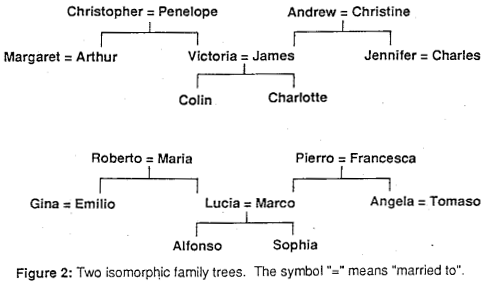
\includegraphics[width = 0.5\textwidth]{../writing/cogsci_2017/figures/hinton_family_tree_figure.png}
    \end{center}
    }
\end{itemize}
\end{frame}

\begin{frame}{Hinton family tree task: Problems}
A few problems:
\begin{itemize}
    \item<1-> Cannot simply ``eyeball'' analogy extraction here, need a principled measure.
    \begin{itemize}
	\item<2-> Use a non-parametric test on each SVD mode to see whether the domains share more analogous structure in this mode than would be expected by chance. 
    \end{itemize}
\end{itemize}
\uncover<2-> {
    \includegraphics[width = \textwidth]{figures/nonparametric_test.png}

}
\note{Hinton shared relationship inputs, and had shared hidden layers, but we want to strip down to see if the analogies will emerge from the learning dynamics like in the above task.}
\end{frame}

\begin{frame}{Results}
Significant amounts of analogy extraction!\\[11pt]
    \uncover<2->{
    First layer input modes:
    \begin{center}
    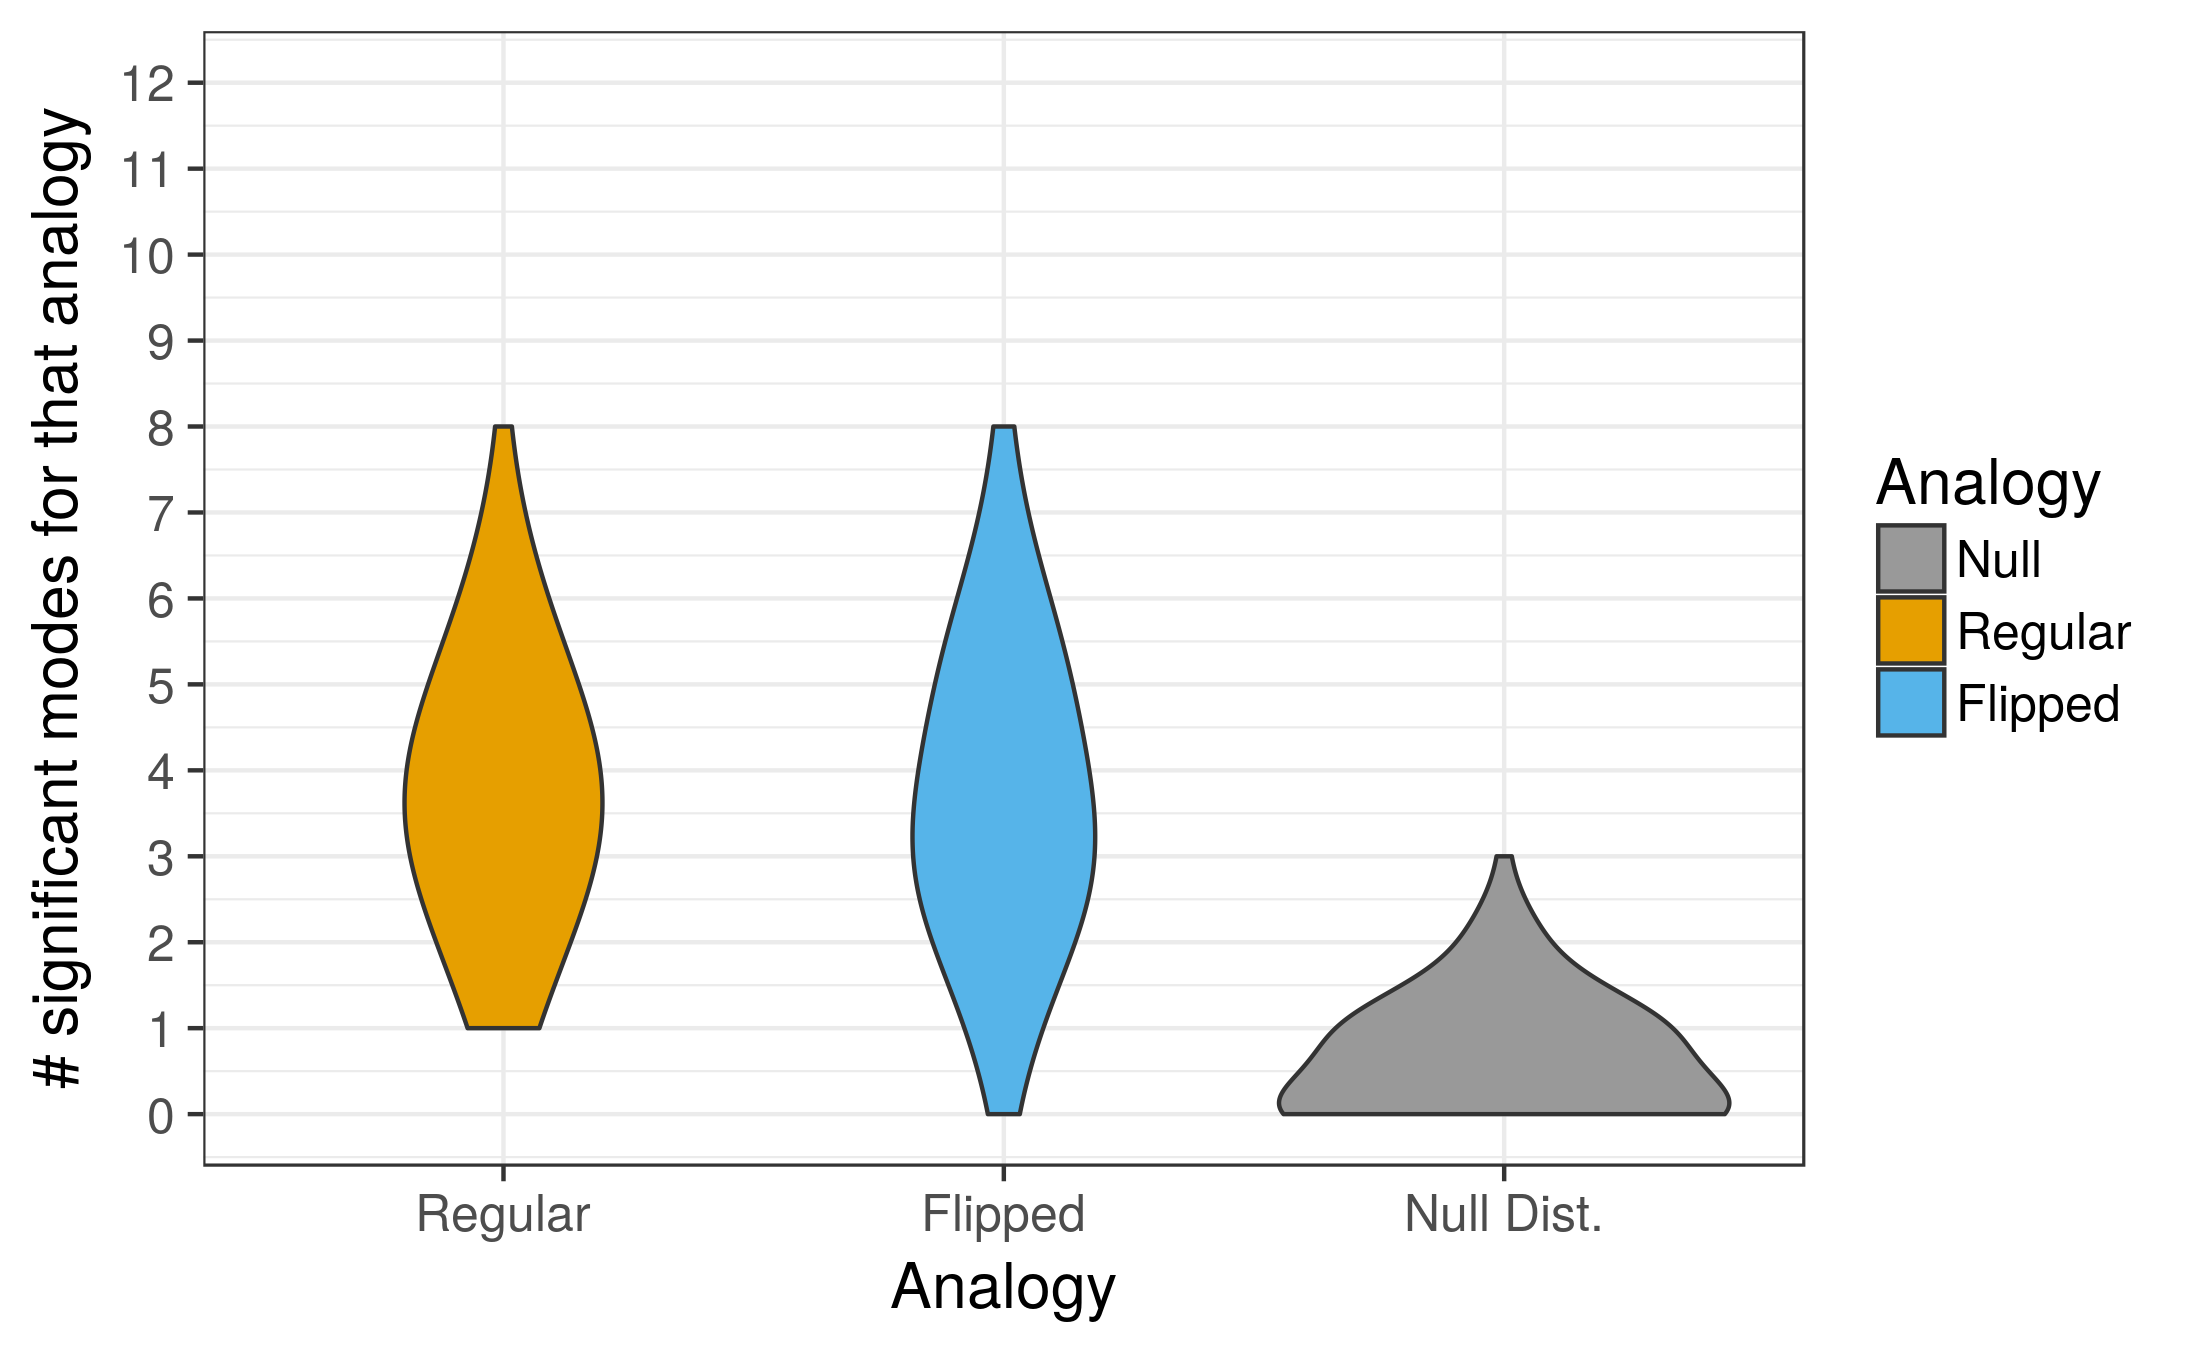
\includegraphics[width=0.75\textwidth]{../hinton_family_tree/results/input_mode_projections_violin.png} 
    \end{center}
    }
\end{frame}
\begin{frame}{Results}
Also in second layer output modes (although slightly less):
\begin{center}
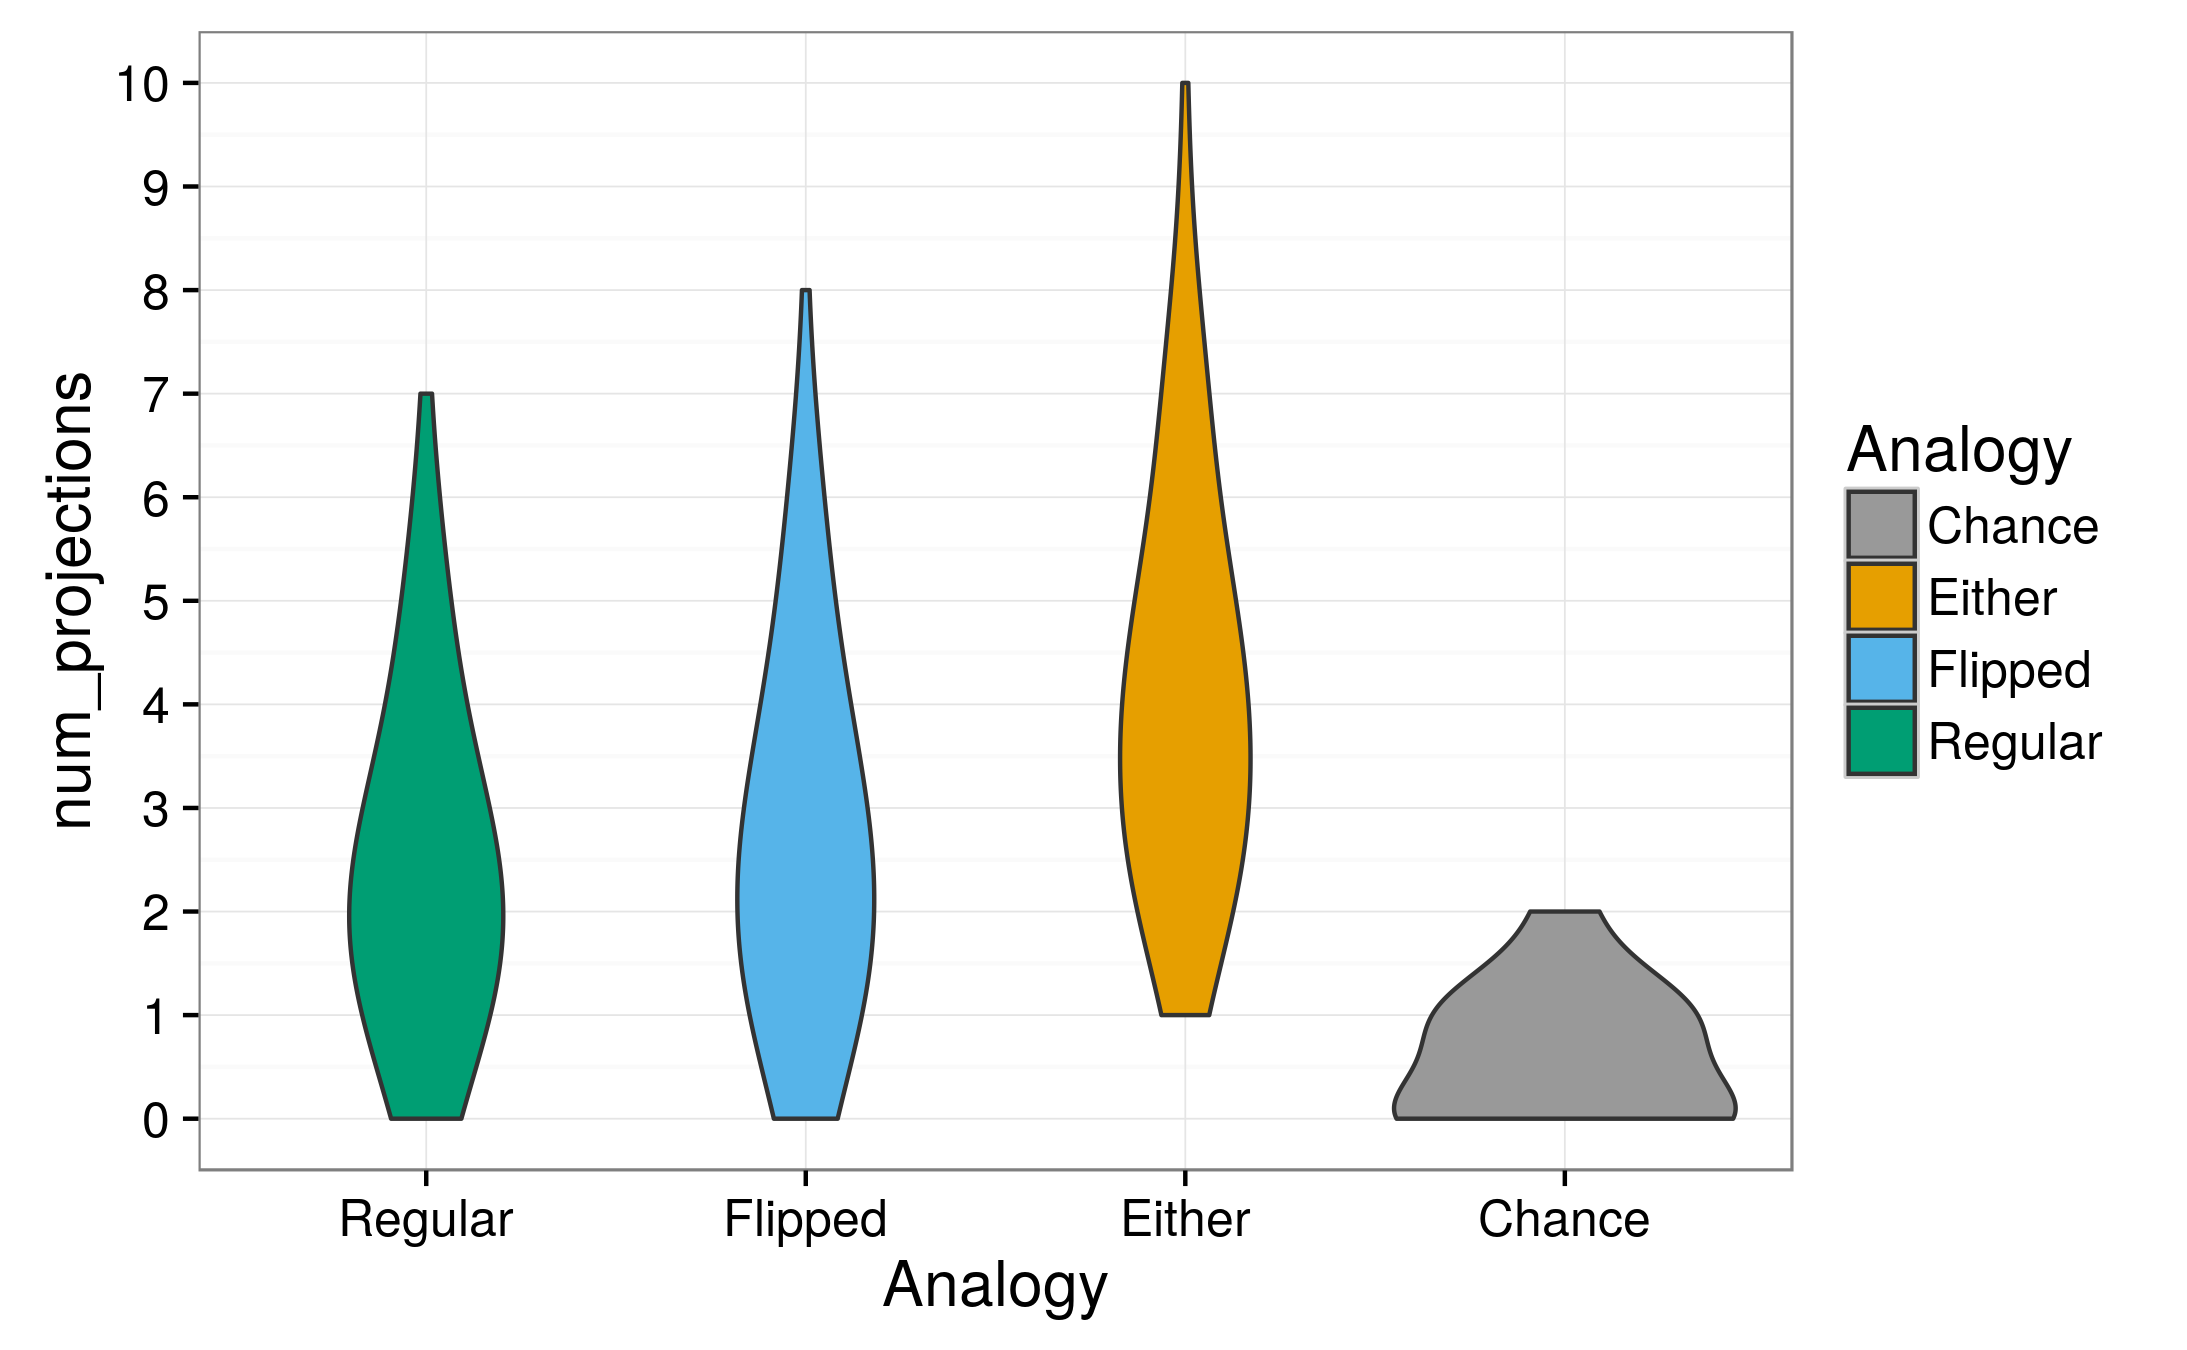
\includegraphics[width=0.75\textwidth]{../hinton_family_tree/results/output_mode_projections_violin.png} 
\end{center}
\end{frame}

\begin{frame}{Highlights:}
The input layers had:
\begin{itemize}
    \item<1-> A median of 6 modes showing significant extraction of the regular or flipped analogy (null: only 0.01\% of runs with 6 significant modes, median 0).
    \item<2-> 3 or more significant components overall in all of the runs (null: in 3\% of runs).
\end{itemize}
\uncover<3->{Analogy extraction appears \textbf{more consistent in a more complex task} than it was in the toy task.}
\end{frame}

\section{Preparation for Future Learning}
\begin{frame}{PFL}
The above required that the tasks are learned simultaneously, but humans need to find analogies beyond things that are simply learned at the same time. There are a few ways we could resolve this: 
\begin{itemize}
\item<2-> Experiences need not be simultaneous if the events can be interleaved on replay, c.f. complementary learning systems \cite{Kumaran2016}.
\item<3-> If we allow some computations to be shared between the tasks, that may also suffice.
\begin{itemize}
\item<4-> Could also allow us to model Preparation for Future Learning (PFL)
\end{itemize}
\end{itemize}
\end{frame}

%%TODO Slide on training

%%TODO: Path explanation
\begin{frame}{PFL}
Suppose we share some weights, can we see evidence of preparation for future learning?\\[11pt]
\begin{columns}
\column{0.45\textwidth}
    \uncover<1->{
    \begin{center}
    \includegraphics[width=\textwidth]{figures/shared_weights_network_diagram.png}
    \end{center}
    }
\column{0.45\textwidth}
    \uncover<2->{\textbf{Yes}, learning is faster after learning an analogous task than after learning a non-analogous one. \vspace{-10pt}
    \begin{center}
    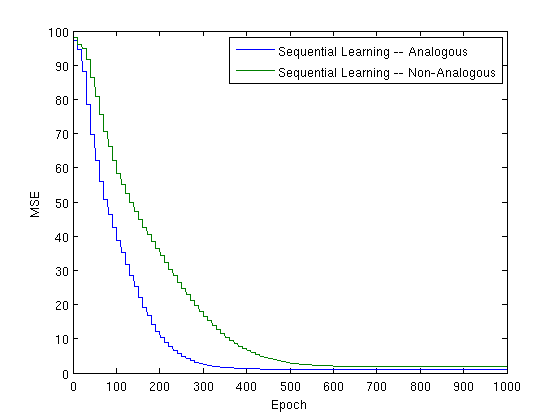
\includegraphics[width=1.1\textwidth]{figures/preparation_for_learning.png} 
    \end{center}
    }
\end{columns}
\note{Would expect this effect to increase with increasing depth of the network}
\end{frame}

\begin{frame}{PFL Results}
This still results in representation of the analogy (when the tasks are analogous). \\[11pt] 
\begin{columns}
\column{0.45\textwidth}
    \uncover<2->{
    Learn analogous task first:
    \begin{center}
    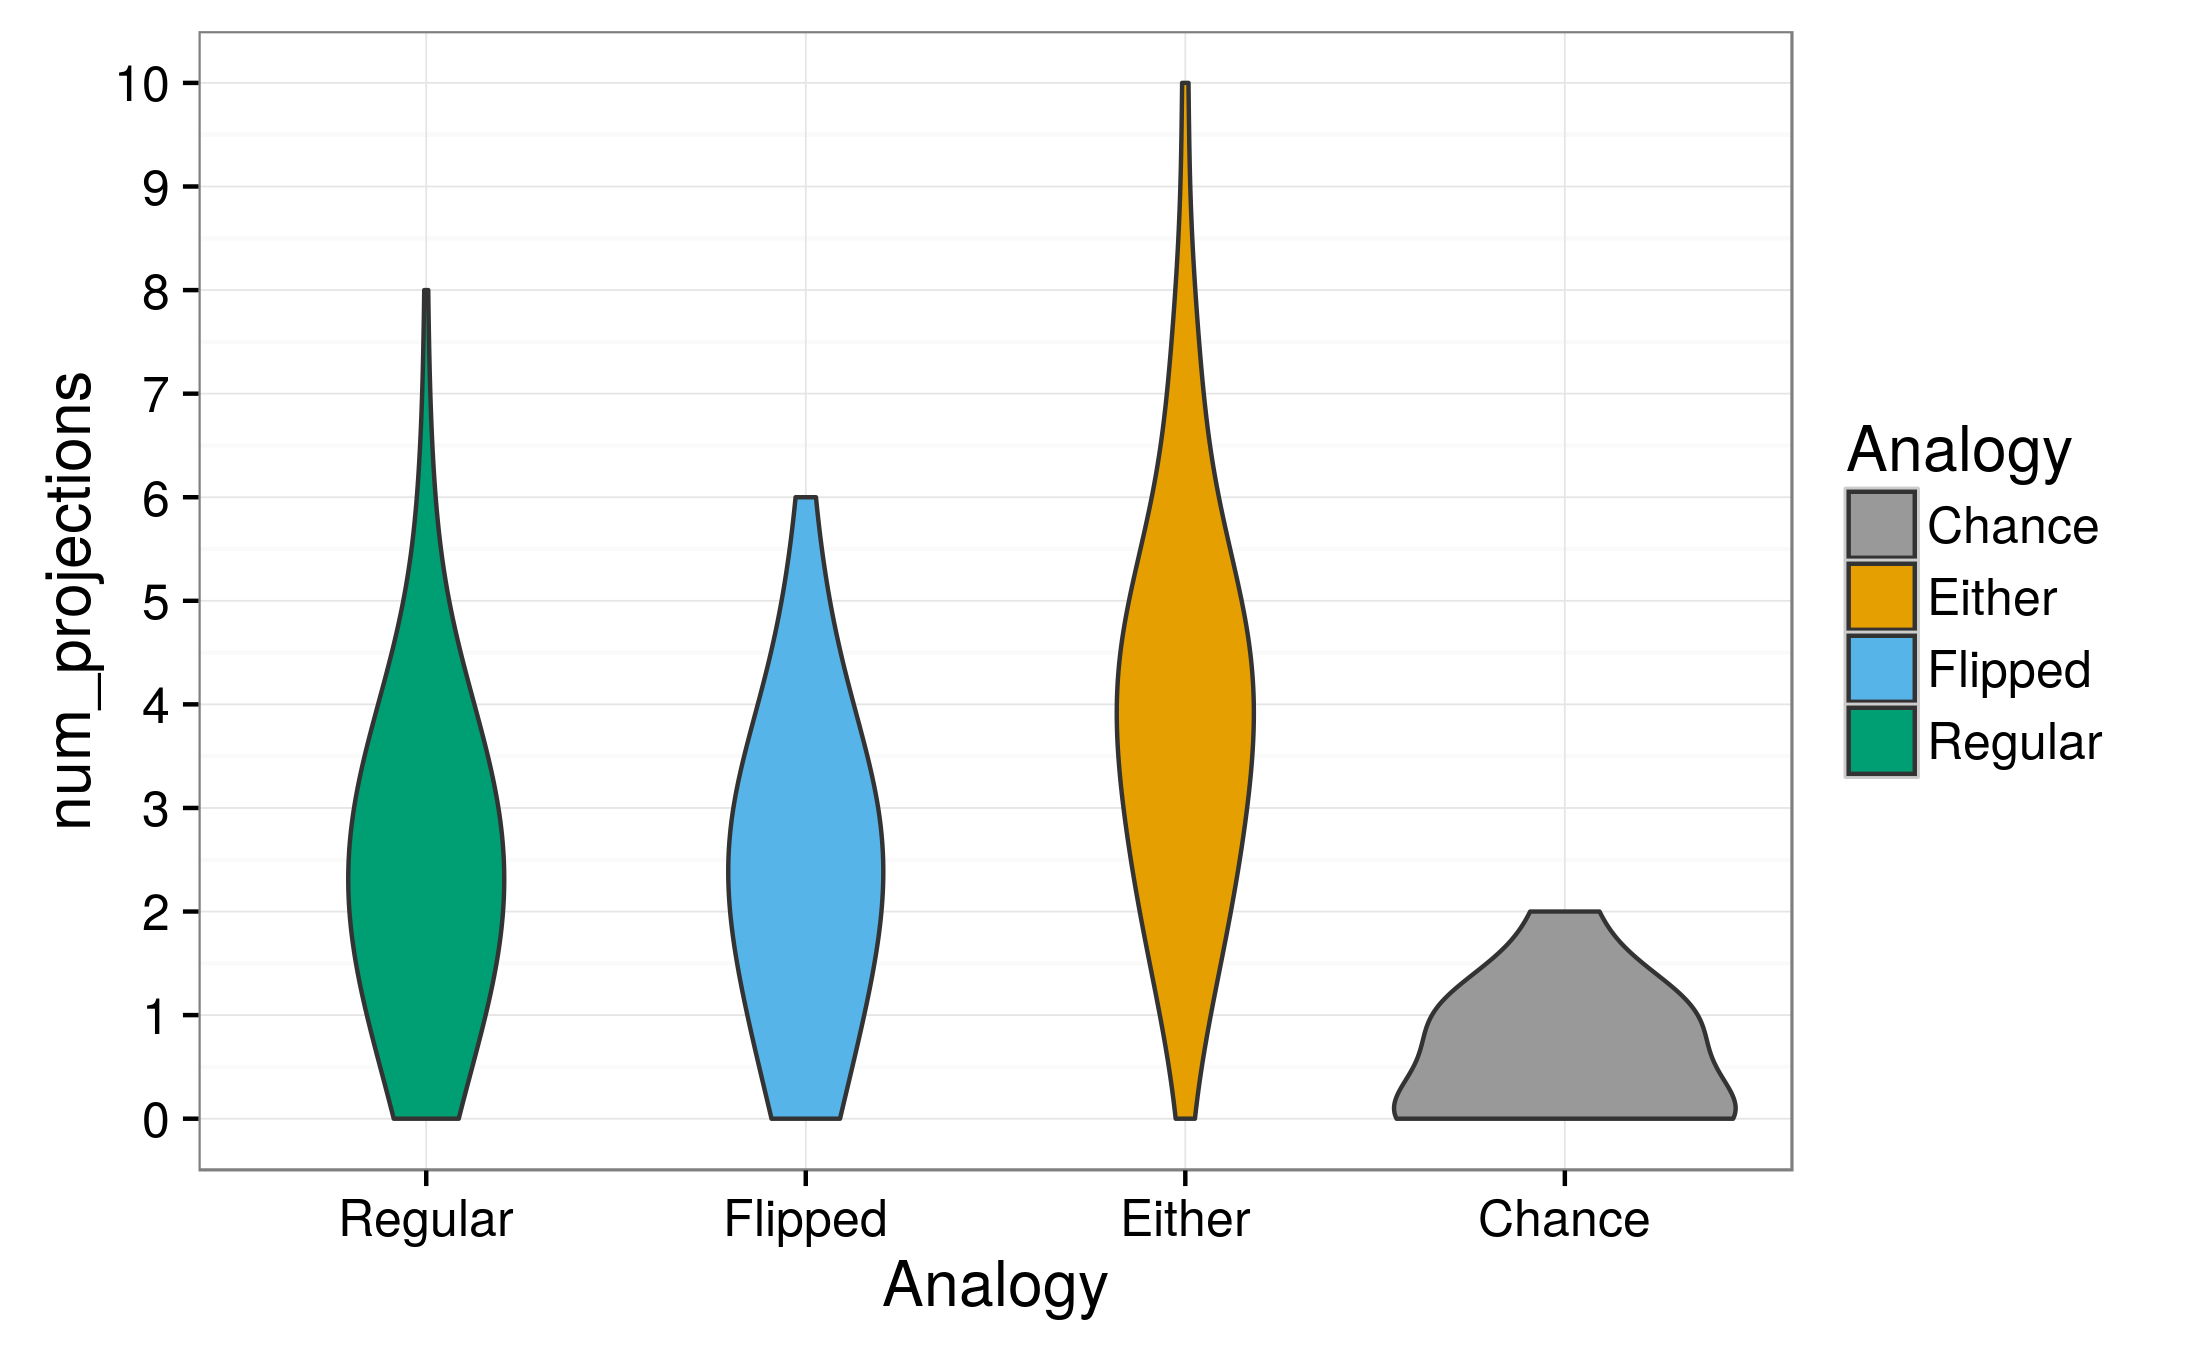
\includegraphics[width=1.2\textwidth]{../hinton_family_tree/results/pfl/anal_input_mode_projections_violin.png}
    \end{center}
    }
\column{0.45\textwidth}
    \uncover<3->{
    Learn different task first:
    \begin{center}
    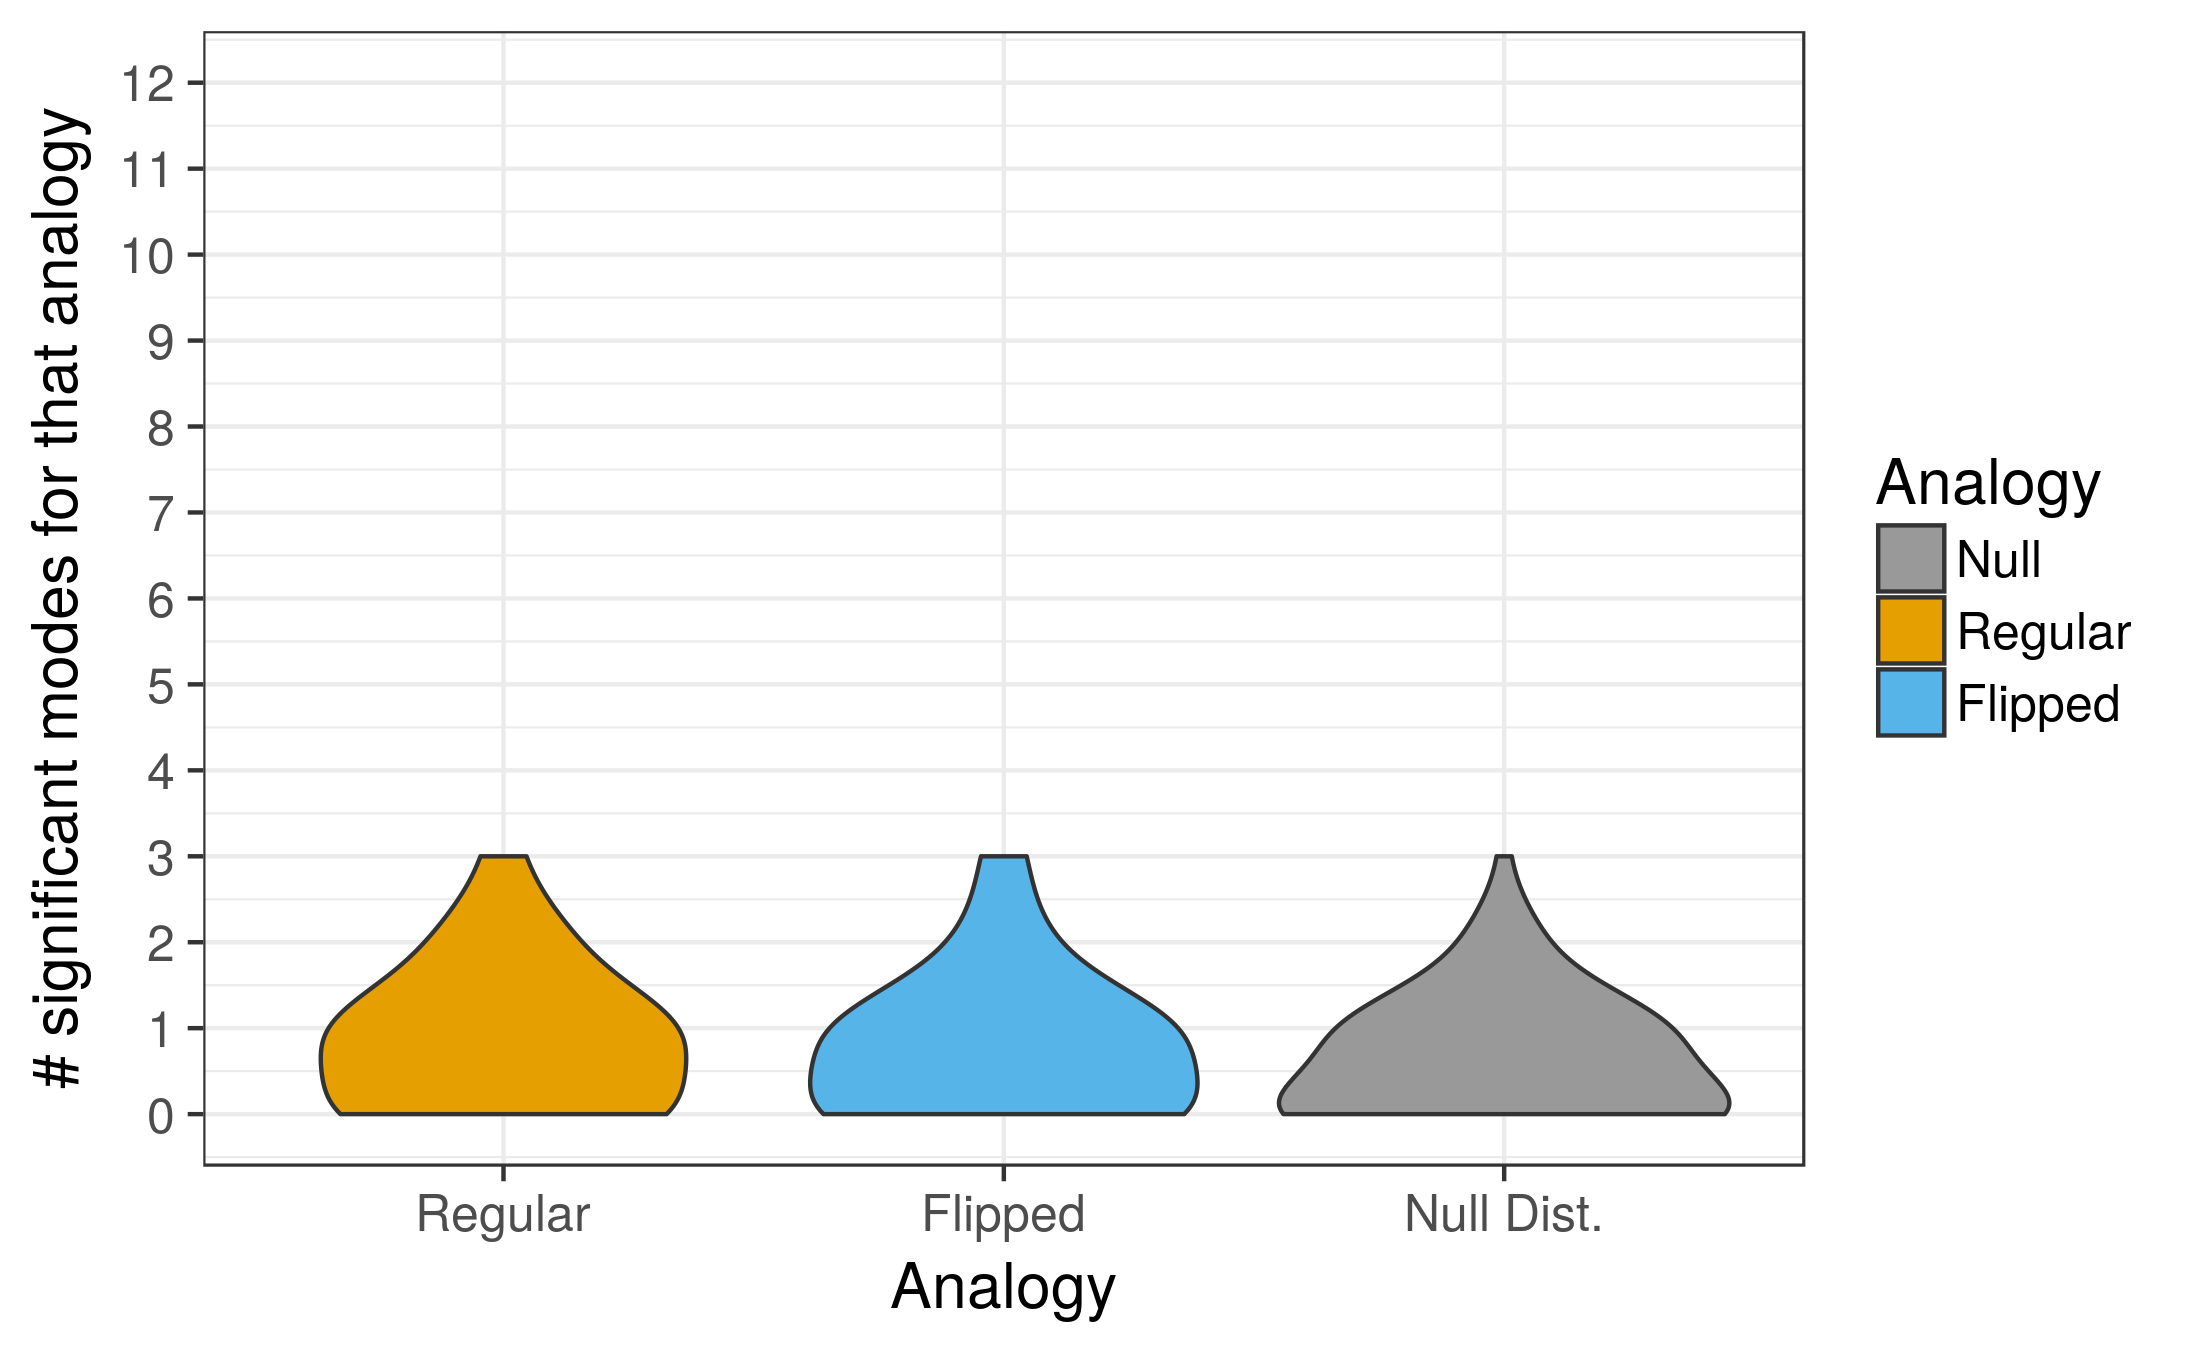
\includegraphics[width=1.2\textwidth]{../hinton_family_tree/results/pfl/alt_input_mode_projections_violin.png}
    \end{center}
    }
\end{columns}
\end{frame}

\section{Conclusions}

\begin{frame}{Results summary}
\begin{itemize}
    \item<1-> We outlined a new linearized analysis method for non-linear neural networks. 
    \item<2-> Used this in a toy task to show that analogies between non-overlapping tasks emerge naturally from learning dynamics. 
    \item<3-> Used in a more complicated task, and found that extraction of the analogies was even more consistent than on the toy task. 
    \item<4-> This extraction of analogies can emerge from:
    \begin{itemize}
	\item<5-> Simultaneous learning (or replay) without shared weights. 
	\item<6-> Non-simultaneous learning with shared weights.
    \end{itemize}
\end{itemize}
\end{frame}

\begin{frame}{Results summary}
This may provide a good model for ``slow'' human analogical reasoning and transfer, including:
\begin{itemize}
    \item<2-> Possible amortized inference about analogies which could potentially support later explicit analogical reasoning.
    \item<3-> Benefits of multiple mutually supporting tasks.
    \item<4-> Transfer as preparation for future learning.
\end{itemize}
\end{frame}

\begin{frame}{Acknowledgements}
Thanks to:
\begin{itemize}
    \item Co-authors: Shaw Hsu \& Jay McClelland
    \item The rest of the lab (especially Arianna) for helpful conversations and feedback. 
    \item Erin, Lester, Mona, Pam, and Yochai, for feedback on this talk.
    \item You, for listening.
\end{itemize}
\end{frame}

\begin{frame}[allowframebreaks]
\bibliographystyle{apacite}
\bibliography{shared_reps}
\end{frame}

\appendix
\begin{frame}{Analogy from gradients}
In toy example, any unit that starts pointing slightly in direction of analogy (as some will due to random initialization) will extract it further when base rates have been learned.\\[11pt]
\begin{columns}
    \column{0.45\textwidth}
    \uncover<1->{Base rates by domain: \phantom{a little shared structure}{\relsize{-1}
    \[
    \left[ \begin{matrix} 
     1 & 1 & 0 & 0 \\ 
     0.5 & 0.5 & 0 & 0 \\
     0.5 & 0.5 & 0 & 0 \\
     0 & 0 & 1 & 1 \\ 
     0 & 0 & 0.5 & 0.5 \\
     0 & 0 & 0.5 & 0.5 \\
    \end{matrix}  \right] 
    \]
    }
    }
    \column{0.45\textwidth}
    \uncover<1->{Base rates + a little shared structure{ \relsize{-1}
    \[
    \left[ \begin{matrix} 
     1 & 1 & 0 & 0 \\ 
     0.6 & 0.4 & 0.1 & -0.1 \\
     0.4 & 0.6 & -0.1 & 0.1 \\
     0 & 0 & 1 & 1 \\ 
      0.1 & -0.1 & 0.6 & 0.4 \\
      -0.1 & 0.1 & 0.4 & 0.6 \\
    \end{matrix}  \right] 
    \] 
    }
    }
\end{columns} 
{ \relsize{-1}
\[
\begin{array}{cccccc||c||cccccc} 
\multicolumn{6}{c||}{\text{output error}}  & \text{unit}  & \multicolumn{6}{c}{\text{unit output weight updates}} \\
\hline
 0 & + & - & 0 & 0 & 0  &   +    &  0 & + & - & 0 & 0 & 0   \\
0 & - & + & 0 & 0 & 0  &   -  & 0 & + & - & 0 & 0 & 0   \\
 0 & 0 & 0 & 0 & + & - &   +   &  0 & 0 & 0 & 0 & + & - \\
 0 & 0 & 0 & 0 & - & +  &  - &  0 & 0 & 0 & 0 & + & - \\
\hline
\multicolumn{7}{r}{\text{net output weight update:}} &   0 & + & - & 0 & + & - \\
\end{array} 
\]
}
\end{frame}

\begin{frame}{Carillon}
\begin{center}
\movie[width=0.33\textwidth,height=0.58\textwidth]{}{harmony_of_zion_clip_rotated.mp4}
\end{center}
\end{frame}


\end{document}
